\documentclass{beamer}
\setbeamertemplate{footline}[page number]
\date{}
\author{}
\institute{}

%%%%%%% Put these names back in the final version 
%\\Aswathy Rajendra Kurup\\Meenu Ajith}
%\institute{Department of Electrical and Computer Engineering\\The University of New Mexico}
\setbeamercovered{transparent}
\usepackage{setspace}
\usepackage{array}
\usepackage[T1]{fontenc}
\usepackage{graphicx}
\usepackage{amsmath}
\usepackage{amsfonts}
\usepackage{amssymb}
\usepackage{makeidx}
\usefonttheme{serif}
\usepackage{multirow}
\usepackage{booktabs} 
\usepackage{rotating}
\usepackage{color}
\usepackage{float}
\usepackage[latin1]{inputenc}
\usepackage[english]{babel}
\usepackage{amsmath}
\usepackage{amsfonts}
\usepackage{eurosym}
\usepackage{rotating}
\usepackage{multicol}
\usepackage{pythonhighlight}
\usepackage[normalem]{ulem}
\newcommand{\ba}{{\bf a}}
\newcommand{\bb}{{\bf b}}
\newcommand{\bc}{{\bf c}}
\newcommand{\bd}{{\bf d}}
\newcommand{\be}{{\bf e}}
\newcommand{\bbf}{{\bf f}}
\newcommand{\bg}{{\bf g}}
\newcommand{\bh}{{\bf h}}
\newcommand{\bi}{{\bf i}}
\newcommand{\bk}{{\bf k}}
\newcommand{\bl}{{\bf l}}
\newcommand{\bm}{{\bf m}}
\newcommand{\bn}{{\bf n}}
\newcommand{\bo}{{\bf o}}
\newcommand{\bp}{{\bf p}}
\newcommand{\bq}{{\bf q}}
\newcommand{\br}{{\bf r}}
\newcommand{\bs}{{\bf s}}
\newcommand{\bt}{{\bf t}}
\newcommand{\bu}{{\bf u}}
\newcommand{\bv}{{\bf v}}
\newcommand{\bw}{{\bf w}}
\newcommand{\bx}{{\bf x}}
\newcommand{\by}{{\bf y}}
\newcommand{\bz}{{\bf z}}

\newcommand{\bA}{{\bf A}}
\newcommand{\bB}{{\bf B}}
\newcommand{\bC}{{\bf C}}
\newcommand{\bE}{{\bf E}}
\newcommand{\bG}{{\bf G}}
\newcommand{\bH}{{\bf H}}
\newcommand{\bI}{{\bf I}}
\newcommand{\bK}{{\bf K}}
\newcommand{\bL}{{\bf L}}
\newcommand{\bM}{{\bf M}}
\newcommand{\bO}{{\bf O}}
\newcommand{\bQ}{{\bf Q}}
\newcommand{\bR}{{\bf R}}
\newcommand{\bS}{{\bf S}}
\newcommand{\bT}{{\bf T}}
\newcommand{\bV}{{\bf V}}
\newcommand{\bW}{{\bf W}}
\newcommand{\bX}{{\bf X}}
\newcommand{\bY}{{\bf Y}}
\newcommand{\bZ}{{\bf Z}}
\newcommand\uptocnt{\stackrel{\mathclap{\normalfont\mbox{c}}}{\propto}}
\newcommand{\bpt}{{\bf pt}}
\newcommand{\bpl}{{\bf pl}}
\newcommand{\bdp}{{\bf dp}}
\newcommand{\btemp}{{\bf temp}}

\newcommand{\bmu}{{\boldsymbol \mu}}
\newcommand{\bSigma}{{\boldsymbol \Sigma}}
\newcommand{\bsigma}{{\boldsymbol \sigma}}
\newcommand{\bvarPhi}{{\boldsymbol \varPhi}}
\newcommand{\bvarphi}{{\boldsymbol \varphi}}
\newcommand{\bPhi}{{\boldsymbol \Phi}}
\newcommand{\bdelta}{{\boldsymbol \delta}}
\newcommand{\bZero}{{\bf 0}}
\newcommand{\bOne}{{\bf 1}}
\newcommand{\balpha}{{\boldsymbol \alpha}}
\newcommand{\bAlpha}{{\boldsymbol A}}
\newcommand{\btheta}{{\boldsymbol \theta}}

\newcommand{\softmax}{\text{softmax}}
\newcommand{\diag}{\text{diag}}
\newcommand{\sinc}{\mathrm{sinc}}
\newcommand{\argmin}{\mathop{\mathrm{argmin}}}
\newcommand{\infl}{\eta}
\newcommand{\Ind}{\mathrm{I}}
\newcommand{\Real}{\mathbb R}
\newcommand{\Intg}{\mathbb Z}
\newcommand{\Complex}{\mathbb C}
\newcommand{\Natural}{\mathbb N}
\newcommand{\Fourier}[1]{\mathcal{F} \{#1\}}
%\newcommand{\ii}{\mathbbm{i}}
\newcommand{\bphi}{\boldsymbol{\mathit{\phi}}}

\newcommand{\hs}{\hspace{2pt}}
\newcommand{\sign}{\text{sign}}
\author{Manel Mart\'inez-Ram\'on\\Meenu Ajith\\Aswathy Rajendra Kurup}

\usetheme{Madrid}
\usecolortheme{beaver}
\usepackage{tikz}
\usetikzlibrary{fit,arrows,calc,positioning}
\usepackage{listings}
\usepackage{xcolor}
\usepackage{emerald} 
\usepackage[T1]{fontenc} 
\usepackage{verbatim}
\usepackage{graphicx}
\usepackage{epsfig}
\usepackage{psfrag}
\usepackage[english]{babel}
\usepackage{listings}
\usepackage{courier}
\usepackage{color}
 \usepackage{vwcol} 
 \usepackage[english]{babel} % To obtain English text with the blindtext package
\usepackage{blindtext}
\definecolor{codegreen}{rgb}{0,0.6,0}
\definecolor{codegray}{rgb}{0.5,0.5,0.5}
\definecolor{codepurple}{rgb}{0.58,0,0.82}
\definecolor{backcolour}{rgb}{0.95,0.95,0.92}

\lstdefinestyle{mystyle}{
  backgroundcolor=\color{backcolour},   commentstyle=\color{codegreen},
  keywordstyle=\color{magenta},
  numberstyle=\tiny\color{codegray},
  stringstyle=\color{codepurple},
  basicstyle=\ttfamily\footnotesize,
  breakatwhitespace=false,         
  breaklines=true,                 
  captionpos=b,                    
  keepspaces=true,                 
  numbers=left,                    
  numbersep=5pt,                  
  showspaces=false,                
  showstringspaces=false,
  showtabs=false,                  
  tabsize=2
}
\lstset{style=mystyle}

%% Stuff for movies

% %\newcommand{\bt}{{\bf t}}
% \newcommand{\br}{{\bf r}}
% \newcommand{\bs}{{\bf s}}
% \newcommand{\by}{{\bf y}}
% \newcommand{\bz}{{\bf z}}
% \newcommand{\bx}{{\bf x}}
% \newcommand{\bw}{{\bf w}}
% \newcommand{\be}{{\bf e}}
% \newcommand{\bbf}{{\bf f}}
% \newcommand{\bb}{{\bf b}}
% \newcommand{\bd}{{\bf d}}
% \newcommand{\bA}{{\bf A}}
% \newcommand{\bB}{{\bf B}}
% \newcommand{\bL}{{\bf L}}
% \newcommand{\bM}{{\bf M}}

% \newcommand{\bC}{{\bf C}}
% \newcommand{\bI}{{\bf I}}
% \newcommand{\bK}{{\bf K}}
% \newcommand{\bk}{{\bf k}}
% \newcommand{\bT}{{\bf T}}
% \newcommand{\bV}{{\bf V}}
% \newcommand{\bW}{{\bf W}}
% \newcommand{\bX}{{\bf X}}
% \newcommand{\bY}{{\bf Y}}
% \newcommand{\bZ}{{\bf Z}}
% \newcommand{\bm}{{\bf m}}
% \newcommand{\bpt}{{\bf pt}}
% \newcommand{\bpl}{{\bf pl}}
% \newcommand{\bdp}{{\bf dp}}
% \newcommand{\btemp}{{\bf temp}}
% \newcommand{\bl}{{\bf l}}
% \newcommand{\bu}{{\bf u}}
% \newcommand{\bmu}{{\boldsymbol \mu}}
% \newcommand{\bSigma}{{\boldsymbol \Sigma}}
% \newcommand{\bLambda}{{\boldsymbol \Lambda}}

% \newcommand{\bsigma}{{\boldsymbol \sigma}}
% \newcommand{\bvarphi}{{\boldsymbol \varPhi}}
% \newcommand{\btheta}{{\boldsymbol \theta}}
% \newcommand{\bZero}{{\bf 0}}
% \newcommand{\balpha}{{\boldsymbol \alpha}}
% \newcommand{\bpi}{{\boldsymbol \pi}}
% \newcommand{\bxi}{{\boldsymbol \xi}}
% \newcommand{\bdelta}{{\boldsymbol \delta}}
\lstset{
	language=Python,
	basicstyle=\footnotesize\ttfamily\color{black},
	commentstyle = \footnotesize\ttfamily\color{red},
	keywordstyle=\footnotesize\ttfamily\color{blue},
	stringstyle=\footnotesize\ttfamily\color{black},
%	columns=fixed,
%	numbers=left,    
	numberstyle=\tiny,
	stepnumber=1,
	numbersep=5pt,
	tabsize=1,
	extendedchars=true,
	breaklines=true,            
	frame=b,         
	showspaces=false,
	showtabs=true,
	xleftmargin=6pt,
	framexleftmargin=6pt,
	framexrightmargin=2pt,
	framexbottommargin=4pt,
	showstringspaces=false      
}

\lstloadlanguages{
         Python
}

%\graphicspath{ {./images/} }  % Figures path - used in graphicx

%\selectcolormodel{cmyk}

\mode<presentation>

\newcommand{\dred}{darkred!90!black}
\newcommand{\written}{\ECFJD\textcolor{cyan!50!white}}
\newcommand{\hlight}{\textcolor{\dred}}
\newcommand{\Ex}{\textcolor{\dred}{Ex. }}

% remove navigation symbols in full screen mode
\setbeamertemplate{navigation symbols}{}  
\setbeamertemplate{blocks}[rounded][shadow=false]
\setbeamercolor{note page}{fg=black}

\setbeamercolor{title}{fg=\dred}
\setbeamercolor{frametitle}{fg=white}
\setbeamercolor{frametitle}{bg=\dred}
\setbeamercolor{structure}{fg=black,bg=white}
\setbeamercolor{background canvas}{bg=white,fg=black}
\setbeamercolor{normal text}{fg=black,bg=white}
\setbeamercolor{item}{fg=red!80!black,bg=white!}
\addtobeamertemplate{block begin}{\setbeamercolor{block title}{fg=white,bg=\dred}
\setbeamercolor{block body}{fg=white,bg=gray}}{}


\usepackage{algorithm,algorithmic}
\usepackage[algo2e]{algorithm2e} 
%\title{Lesson 1.1}
\title{2. Training practicalities}
\subtitle{2.2 Optimizers}


\begin{document}

\maketitle

\begin{frame}{Gradient descent}
The basic optimization technique is the gradient descent. 
\begin{itemize}
    \item Stochastic gradient descent (SDG): the gradient is estimated with one sample at a time.
    \item Gradient descent (GD):  the gradient is estimated with a batch of data.  
\end{itemize}
\begin{multicols}{2}
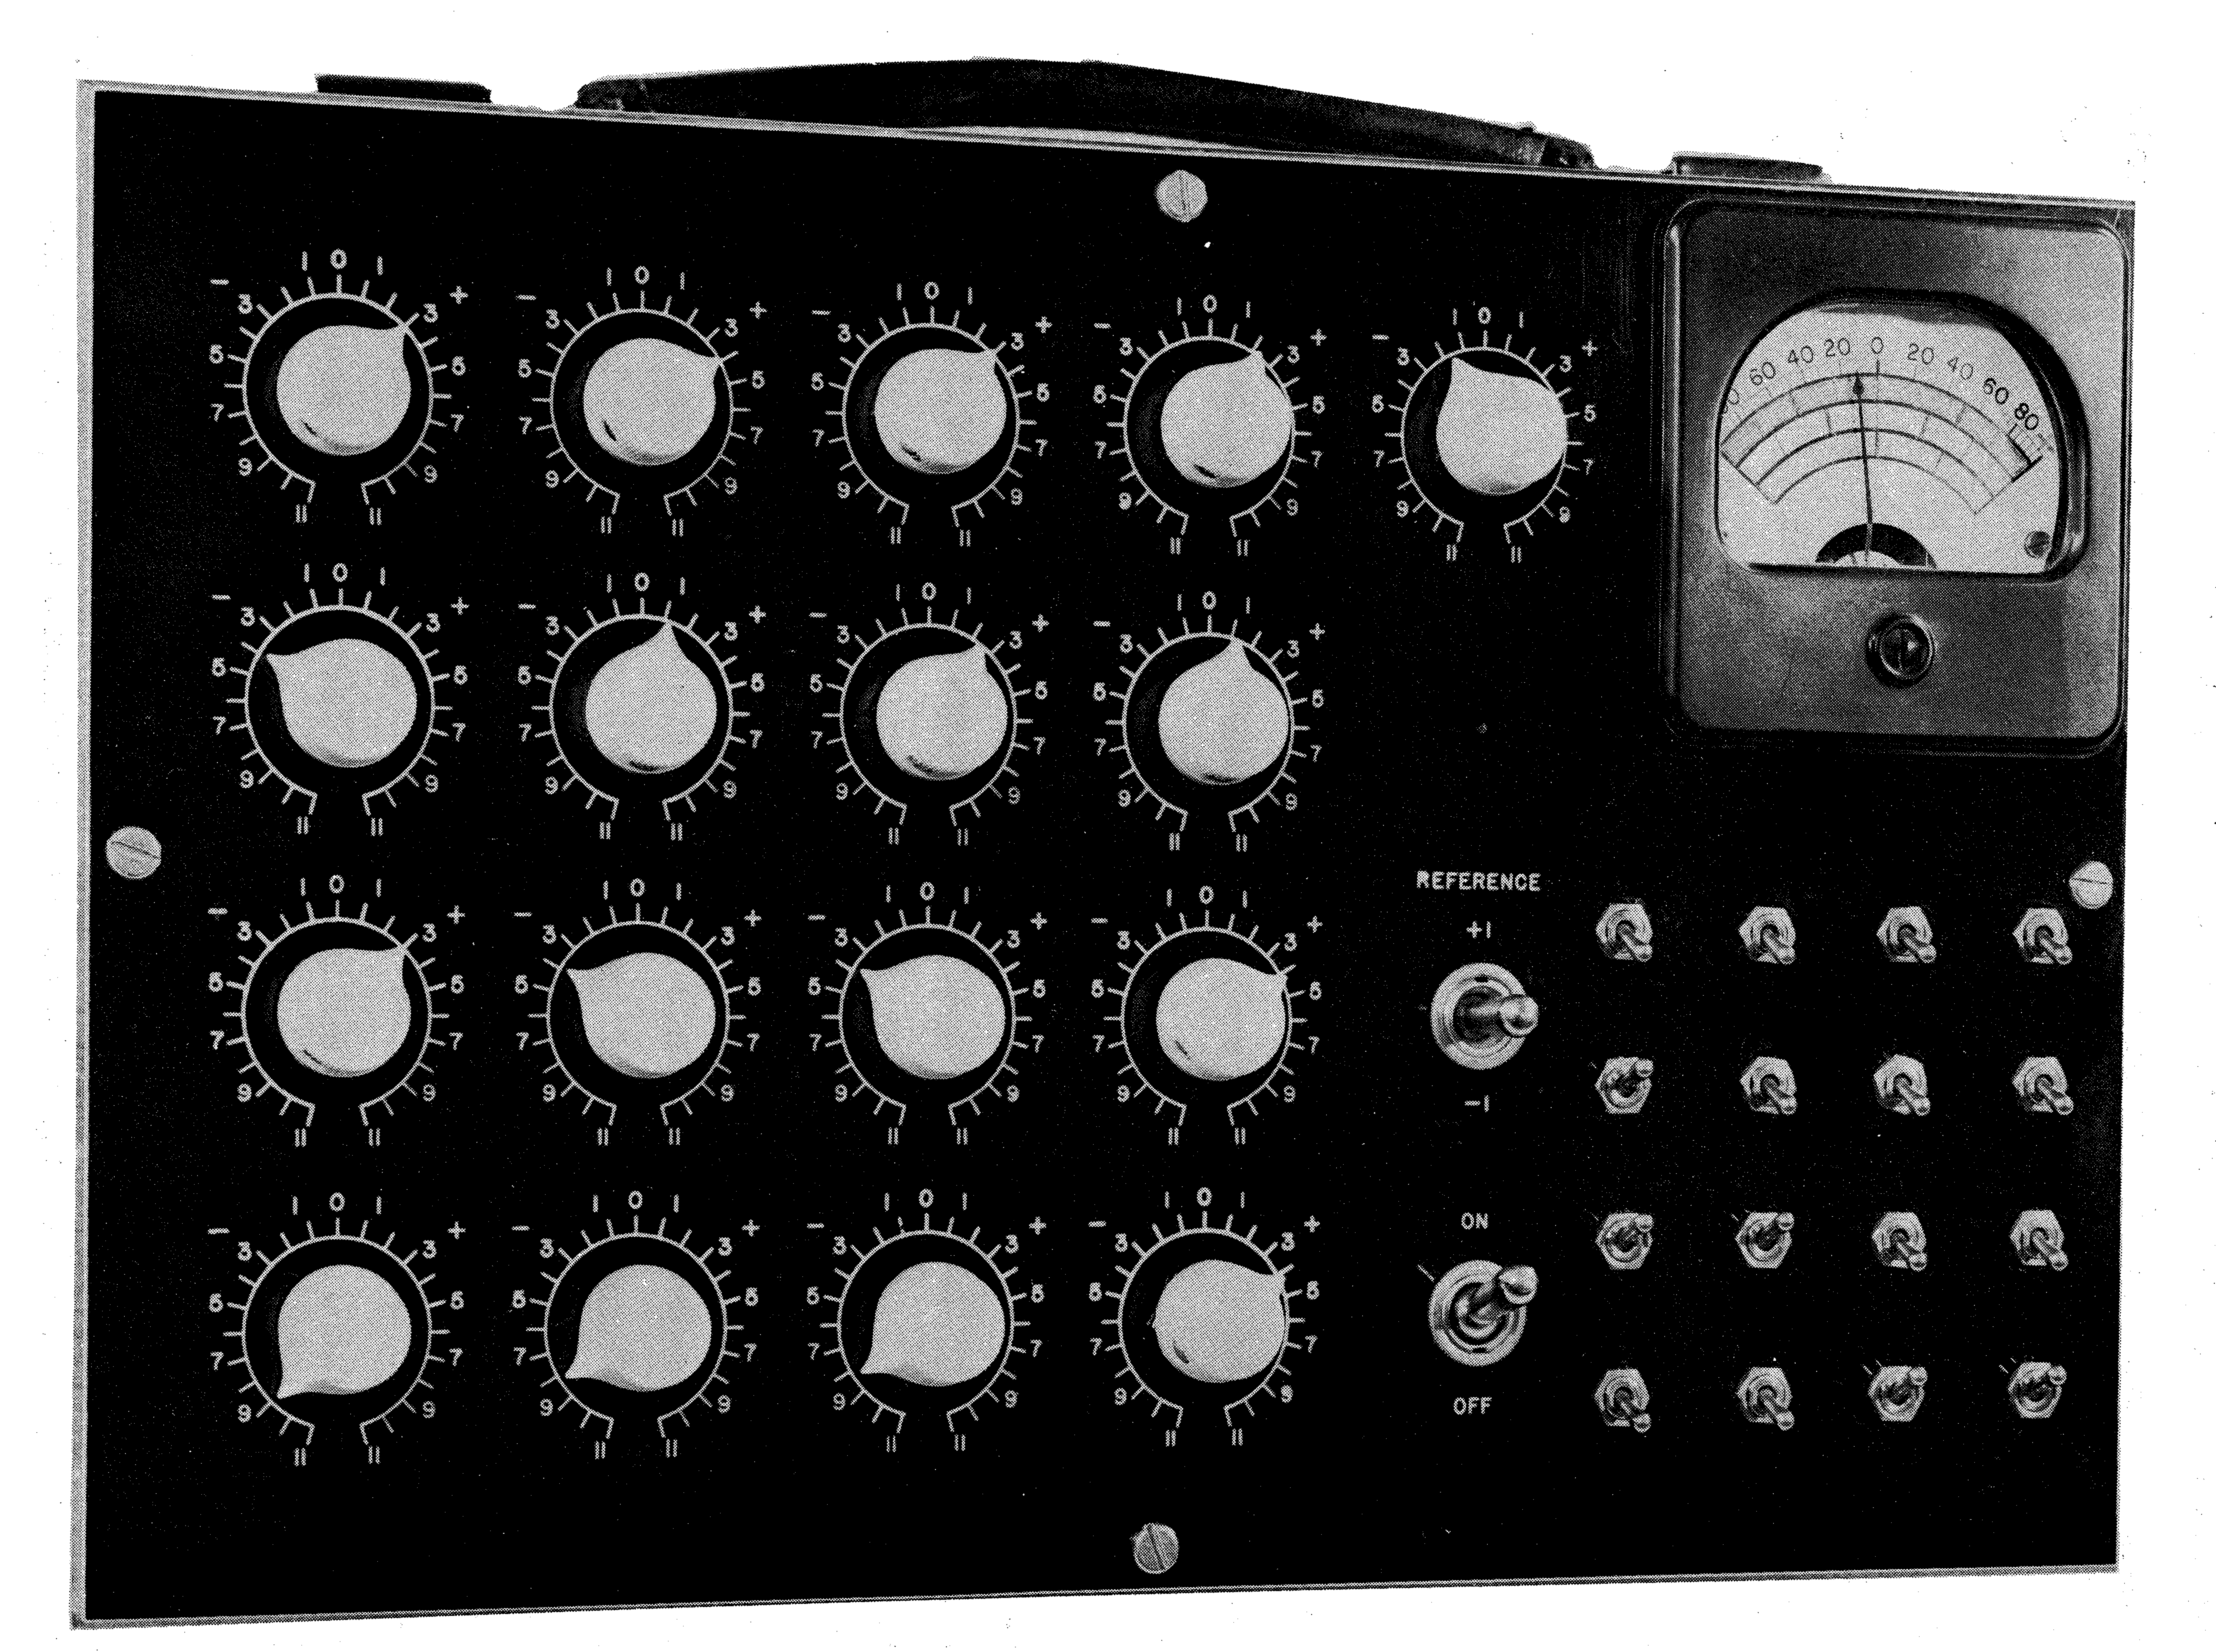
\includegraphics[scale=0.05]{Module 1 (NN)/pics/adaline.pdf}

\columnbreak
\begin{itemize}
\item The Adaline (figure) was the first machine to be trained with SDG. The device consisted of a neuron with a sign activation. The training used the LMS algorithm.

\item Modified 1$^\text{st}$ order algorithms have been proposed that improve the SG.

\end{itemize}
\end{multicols}
\end{frame}

\begin{frame}{Momentum optimization}
    \begin{itemize}
        \item Assume (without loss of generality) that a set of weights are arranged as a vector $\bw$ simulating the position of a particle in a space, with initial velocity $\bv_0=0$.
        \item With a given acceleration $\ba(t)$ applied to the particle, the velocity will be
        $$
        d\bv =  \ba(t) d t
        $$
    \item Now, if the medium has viscosity $\eta$, there will be a deceleration proportional to  the velocity, as
   $$
        d \bv(t) =  -\eta \bv(t)  + \ba(t) dt
    $$
    \end{itemize}
\end{frame}

\begin{frame}{Momentum optimization}

By discretizing the differential equations we obtain

$$
\Delta\bv_{k+1} = -\eta \bv_k + \ba_k \Delta t 
$$
$$
\bv_{k+1} = \gamma \bv_k + \ba_k  
$$
which is obtained by assuming $\Delta t =1$ and $\gamma = 1-\eta$
\begin{multicols}{2}
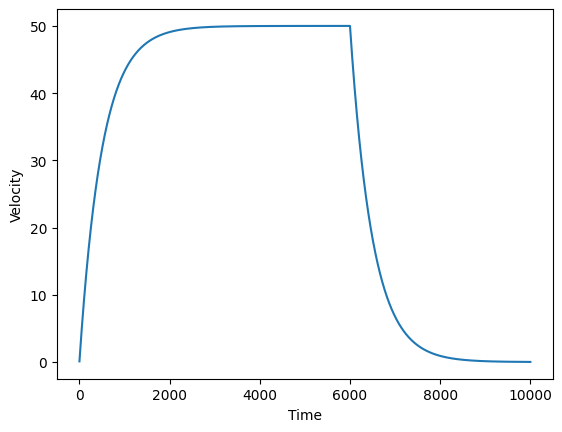
\includegraphics[scale=0.3]{Module 1 (NN)/pics/viscosity.png}

Example: A particle is applied a force $F=mg$ where $g=0.1$ in a viscous fluid. The particle has a viscosity coefficient $\gamma=0.002$. At $t=6000$, the force is suppressed.  

\columnbreak

\end{multicols}
\end{frame}


\begin{frame}{Momentum optimization}

This can be applied to optimization, by assuming that the particle is on the cost function surface and that the acceleration is proportional to the gradient (the slope of the surface). The velocity of the particle is
$$
\bv_{k} = \gamma\bv_{k-1} - \mu \nabla_{\bw} J(\bw_{k}) 
$$

and its position is the integral of the velocity

$$
\bw_{k+1} = \bw_0 + \sum_{k'=0}^k \bv_{k'} = \bw_{k} + \bv_k
$$
\end{frame}



\begin{frame}{Nesterov Accelerated gradient}

When the gradient is zero, the Momentum optimization will still have a velocity. The approach introduced by Yuri Nesterov (1983)  computes the gradient one step ahead to modify the velocity. 
\begin{multicols}{2}
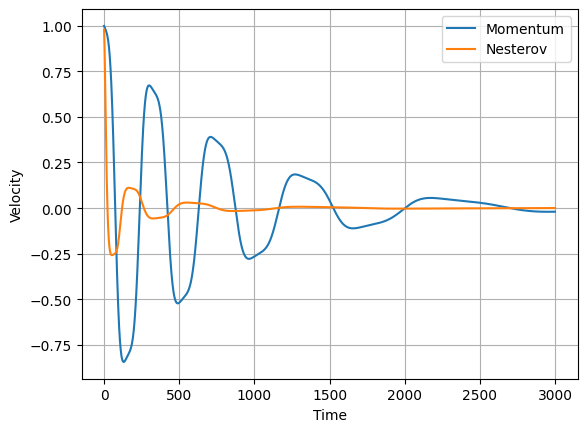
\includegraphics[scale=0.3]{Module 1 (NN)/pics/nesterov.png}

Velocity of the particle around a minimum of the cost function using the Momentum and the Nesterov optimizers.

\columnbreak

Assuming a present position $\bw_k$ and velocity $\bv_k$, the next position is computed as  
$$\tilde{\bw}_{k+1}  = \bw_{k} + \bv_k$$
from which the velocity is modified 
    $$\bv_k = \gamma \bv_{k-1} - \mu \nabla_{\bw}J(\tilde{\bw}_k)$$ 
and then the position is updated
$$    \bw_{k+1}  = \bw_k + \bv_k $$
\end{multicols}

\end{frame}

\begin{frame}{Root Mean Square Propagation (RMSProp)}
The RMSProp adapts the learning rate of each of the weights by an average of the squared norm of the corresponding component of the weight through a decaying window:

$$
\bg_k = \beta \bg_{k-1} + \left(1-\beta\right) \nabla_{\bw}J(\bw_{k}) \odot \nabla_{\bw}J(\bw_{k})
$$

Each weight is updated as 

$$w_{i,k+1} = w_{i,k} - \frac{\mu}{\sqrt{g_{i,k}}+\varepsilon} \left[\nabla_{\bw}J(\bw_{k})\right]_i$$

\end{frame}

\begin{frame}{Adaptive Momentum Estimation (Adam)}

It is a combination of the Momentum and the RMSProp optimizers. First, a velocity is computed as

$$\bv_{k} = \beta_1\bv_{k-1} +(1-\beta_1) \nabla_{\bw} J(\bw_{k}) $$
and then an average of the square norm of each component of the gradient
$$\bg_k = \beta_2 \bg_{k-1} + \left(1-\beta_2\right) \nabla_{\bw}J(\bw_{k}) \odot \nabla_{\bw}J(\bw_{k})$$
\end{frame}

\begin{frame}{Adaptive Momentum Estimation (Adam)}

Then, these  magnitudes are unbiased 
\begin{equation}\nonumber
    \begin{split}
        \tilde{\bv}_k & = \frac{\bv_k}{1-\beta_1^{k}}\\
        \tilde{\bg}_k & = \frac{\bg_k}{1-\beta_2^{k}}\\
    \end{split}
\end{equation}
This is justified by seeing that the facts $\beta_1$ and $\beta_2$ produce a bias in the magnitudes.
\end{frame}


\begin{frame}{Adaptive Momentum Estimation (Adam)}

Finally, each element of the weight vector $\bw_k$ is updated as 
\begin{equation}\nonumber
    w_{i,k+1} = w_{i,k} -\mu \frac{\hat{v}_{i,k}}{\sqrt{\hat{g}_{i,k}}+\varepsilon} 
\end{equation}

\vspace{1cm}

\begin{multicols}{2}

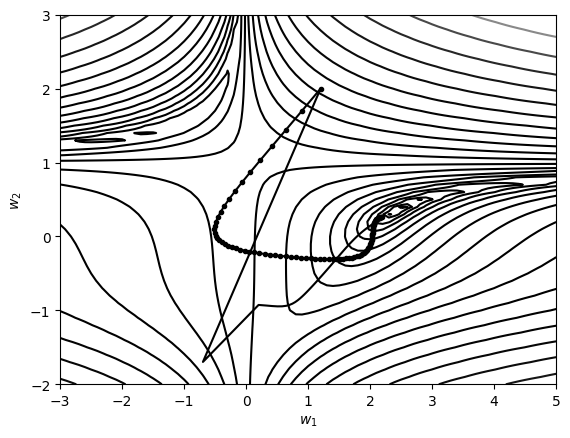
\includegraphics[scale=0.4]{Module 1 (NN)/pics/Adam.png}

\columnbreak

The authors of the algorithm suggest in (Kingma and J. Ba 2014)  to set  the parameters at values $\beta_1=0.9$,  $\beta_2=0.999$ and $\varepsilon = 10^{-8}$. The robustness of this choice is shown in a variety of experiments. However, in some circumstances, these values may need to be cross-validated.   

\end{multicols}
    
\end{frame}

\end{document}

